\documentclass{article}
\usepackage[utf8]{inputenc}
\usepackage[russian]{babel}
\usepackage{amsmath}

\usepackage{graphicx}
\graphicspath{ {jpg/} }
\DeclareGraphicsExtensions{.pdf,.png,.jpg}
\usepackage{float}
\usepackage{subcaption}

\makeatletter
\renewcommand{\@oddfoot}{\hfill\thepage}
\makeatother

\begin{document}
\begin{titlepage}

\thispagestyle{empty}

\begin{center}
\large ФЕДЕРАЛЬНОЕ ГОСУДАРСТВЕННОЕ БЮДЖЕТНОЕ \linebreak
ОБРАЗОВАТЕЛЬНОЕ УЧРЕЖДЕНИЕ \\ ВЫСШЕГО ОБРАЗОВАНИЯ \\
"МОСКОВСКИЙ ГОСУДАРСТВЕННЫЙ УНИВЕРСИТЕТ \\ имени М.В.ЛОМОНОСОВА"
\end{center}

\vfill

\centerline{\Large{\textbf{Изменение яркости пикселей картинки}}}


\vfill
\vfill
\centerline{\textit{Работу выполнил: \hfill студент 224 группы Репин Михаил Денисович}}
\vspace{3mm}
\centerline{\textit{Преподаватель: \hfill Почеревин Роман Владимирович}}

\vfill

\centerline{Москва, 2022}
\clearpage
\end{titlepage} 

\tableofcontents{}
\newpage
\section{Постановка задачи}
\large{Условие: }Программа должна загрузить изображения из графических файлов {\it InputFile1} и  {\it InputFile2 }(размеры входных файлов должны совпадать), изменить яркость каждого пиксела первого изображения так, чтобы она равнялась бы яркости соответствующего пиксела второго изображения и вывести получившееся изображение в графический файл {\it OutputFile}.
Под яркостью пиксела подразумевается сумма компонент всех трех компонент пиксела.
\section{Используемые модули}
Используются: функции  {\bf imwrite} и {\bf imread} из модуля \large{\it imageio.v2}; {\bf unit8}  из модуля \large{\it numpy} для перевода графических файлов из формата .bmp в вид трёхмерной матрицы.
Так же используется функция {\bf argv} из модуля \large{\it  sys}, для получения аргументов командной строки.
\section{Алгоритм}
С помощью функции {\bf imread} считываем данные из двух bmp картинок, полученных на входе, в двумерные массивы \large{\it im1} и \large{\it im2}, каждый элемент которых содержит 3 числа. Считываем длину и высоту этих массивов и сравниваем их, так как по условию размеры изображений должны совпадать. В случае несовпадения размеров выбрасываем исключение \large{\it SystemExit} и завершаем программу с предупреждением: \large{\it Sizes are not equal!}. Иначе, создаем массив \large{\it im3}, в который будут записаны данные для итогового изображения. Но условие, что яркость пикселей изображения на выходе должна равняться яркости соответсвующего пиксела второй картинки не задает однозначно компоненты цветов. Поэтому, будем считать новые значения компонент пиксела, сохраняя их исходные отношения, используя их веса:
\begin{equation*}
v_{i} =  \displaystyle{{x_{i}}\over{x_{1} +x_{2}+x_{3}}} \; \text{\small{\hspace{2mm} , где $x_{i}$ - соответствующая компонента; $i=1 \dots 3$}}\;
\end{equation*}
\newpage
Затем считаем яркость для пикселей второй картинки:
\begin{equation*}
B = y_{1} +y_{2}+y_{3} \; \text{\small{\hspace{2mm} , где $y_{i}$ - соответствующая компонента; $i=1 \dots 3$}}\;
\end{equation*}
Вычисляем новые компоненты пикселей для первой картинки:
\begin{equation*}
x_{i} =   v_{i}*B
\end{equation*}
И окончательно, создаем итоговую картинку \large{\it res.bmp}, куда записываем данные с помощью функции {\bf imwrite}.
 \newpage
\begin{figure}[H]
\section{Примеры использования}
\begin{subfigure}[t]{0.325\linewidth}
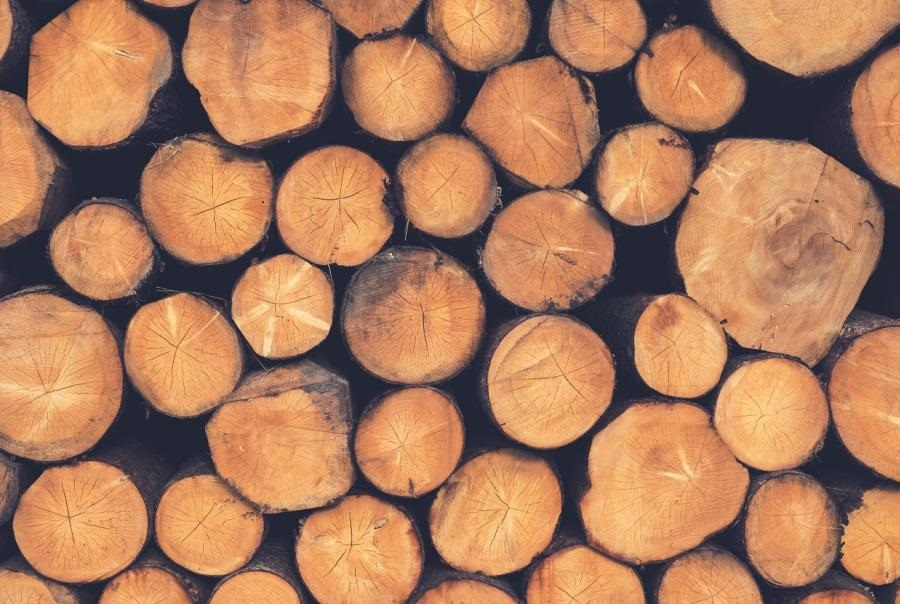
\includegraphics[width=115pt,height=115pt]{1.jpg}
\caption{1.bmp}
\end{subfigure}
\begin{subfigure}[t]{0.325\linewidth}
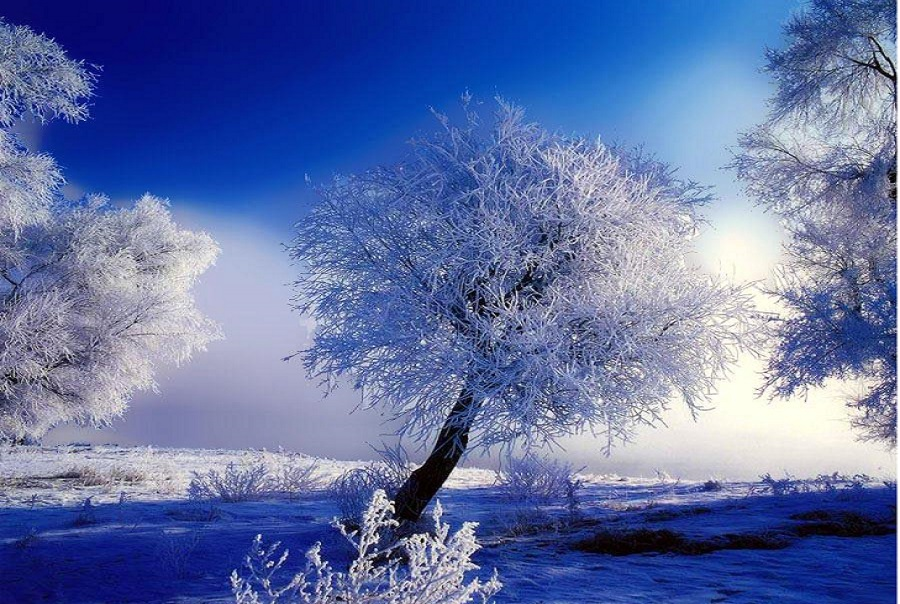
\includegraphics[width=115pt,height=115pt]{2.jpg}
\caption{2.bmp}
\end{subfigure}
\begin{subfigure}[t]{0.325\linewidth}
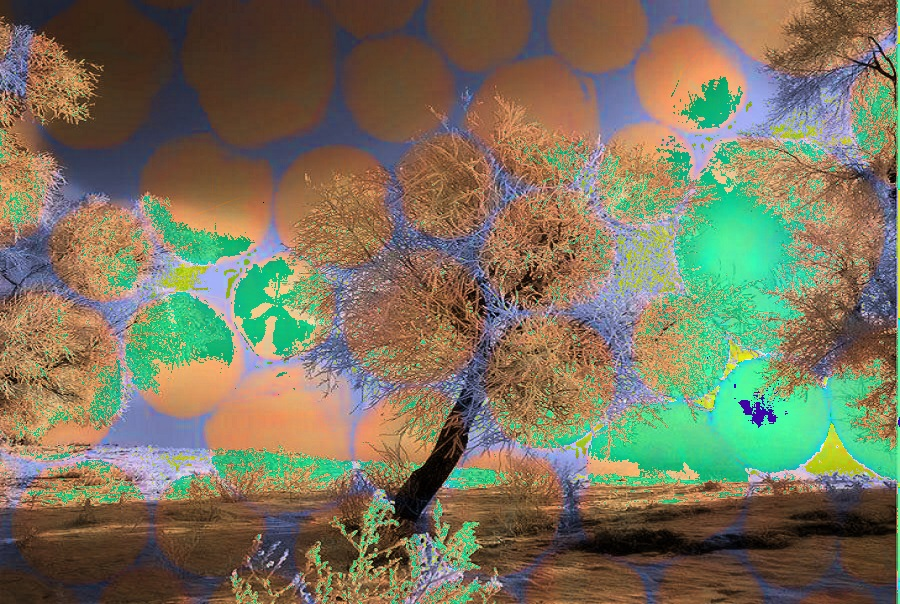
\includegraphics[width=115pt,height=115pt]{res.jpg}
\caption{res.bmp}
\end{subfigure}
\end{figure}

  
\end{document}